\documentclass{article}

\usepackage{arxiv}

\usepackage[utf8]{inputenc}
\usepackage[T1]{fontenc}
\usepackage{hyperref}
\usepackage{url}
\usepackage{booktabs}
\usepackage{amsfonts}
\usepackage{nicefrac}
\usepackage{microtype}
\usepackage{cleveref}
\usepackage{graphicx}
\usepackage{natbib}
\usepackage{doi}
\usepackage{multirow}
\usepackage{adjustbox}

\renewcommand{\headeright}{A Preprint}
\renewcommand{\undertitle}{A Preprint}
\renewcommand{\shorttitle}{Mapping AI-Driven Economic Transformation: A Multi-LLM Delphi Analysis of First-, Second-, and Third-Order Effects Across Industry Verticals}

\title{Mapping AI-Driven Economic Transformation: A Multi-LLM Delphi Analysis of First-, Second-, and Third-Order Effects Across Industry Verticals}

% TODO: Add authors
\author{Author Name \\
Affiliation \\
\texttt{email@example.com}}

\hypersetup{
  pdftitle={Mapping AI-Driven Economic Transformation: A Multi-LLM Delphi Analysis of First-, Second-, and Third-Order Effects Across Industry Verticals},
  pdfkeywords={artificial intelligence, general-purpose technology, Delphi method, scenario analysis, economic transformation, large language models, foresight methodology, sociotechnical transitions},
}

\begin{document}
\maketitle

\begin{abstract}
Artificial intelligence is widely characterized as a general-purpose technology, yet existing research on its economic impact remains bifurcated between micro-level task-substitution studies and macro-level productivity analyses. What is missing is a systematic, cross-sector mapping of cascading transformation effects -- from immediate task automation through structural reorganization to systemic geopolitical consequences. This paper addresses the gap with two contributions. First, it introduces the \textbf{Multi-LLM Delphi} method, in which seven frontier large language models (Claude, GPT-4o, Gemini 2.5 Pro, Grok 3, DeepSeek R1, Qwen Max, and Mistral Large) are queried in parallel with an identical structured prompt, producing independent scenario analyses that are subsequently consolidated through consensus scoring. Second, it applies this method to map AI-driven economic transformation across eight GICS-aligned industry verticals, four sequential adoption stages, three bounding scenarios (MILD, BASE, MAX), and three orders of effects, yielding a 288-cell analytical matrix. Structured comparative content analysis of the 114,000-word corpus reveals six high-consensus convergence zones where five or more models agree -- including labor market bifurcation, infrastructure bottleneck repricing, and the collapse of intermediary business models -- alongside contested futures where model families diverge along identifiable geopolitical lines. US-origin models (Claude, GPT-4o, Gemini, Grok) systematically emphasize market-driven disruption and platform concentration; the Chinese-origin models (DeepSeek, Qwen) foreground state-steered industrial policy and infrastructure sovereignty; the European-origin model (Mistral) privileges regulatory frameworks and social equity. The paper frames these findings through General Purpose Technology theory and the Multi-Level Perspective on sociotechnical transitions, contributing both a novel methodological instrument for scalable foresight research and the most comprehensive cross-sector scenario matrix of AI-driven economic transformation to date. Limitations of the seven-model panel and directions for validation through longitudinal multi-round designs are discussed.


---
\end{abstract}

\keywords{artificial intelligence \and general-purpose technology \and Delphi method \and scenario analysis \and economic transformation \and large language models \and foresight methodology \and sociotechnical transitions}


\textbf{Tobias-Benedikt Blask}

\textit{[Institutional Affiliation]}

---


\subsection{1. Introduction}
\label{sec:1_introduction}

In 2024, over 78 percent of organizations worldwide reported using artificial intelligence in at least one business function, a figure that had doubled in less than two years \citep{chatterji2025chatgpt}. Global investment in AI infrastructure surpassed three hundred billion dollars in combined hyperscaler capital expenditure, and data center electricity demand was projected to more than double by 2030 \citep{iea2024electricity}. These figures signal that AI is no longer an emerging technology but an active force reshaping the productive apparatus of the global economy. Yet the scholarly understanding of \textit{what, precisely, this reshaping will look like} across sectors, stages, and systemic levels remains fragmented.

The fragmentation reflects a structural limitation in the literature. Labor economists model task-level substitution (Acemoglu and Restrepo, 2018, 2019; Acemoglu et al., 2022; Eloundou et al., 2023; Autor, 2024; Frank et al., 2019) and provide rigorous estimates of exposure but typically bracket the structural and systemic consequences that unfold once substitution reaches scale. Management scholars examine firm-level adoption dynamics \citep{raisch2021automation, kanbach2023genai, dwivedi2023chatgpt} but rarely extend analysis to cross-sector convergence effects or geopolitical restructuring. Foresight researchers employ Delphi studies and scenario analysis to map transformation pathways \citep{culot2020manufacturing, fritschy2019autonomous}, but their human expert panels are limited in scale, subject to desirability bias \citep{ecken2011desirability}, and constrained by the availability and self-selection of panelists \citep{foerster2014delphipanel, sokolov2025delphias}.

What is missing is an analytical framework that (a) traces effects across multiple orders of consequence -- from immediate task automation (first order) through structural reorganization of industries, value chains, and labor markets (second order) to systemic geopolitical and civilizational transformation (third order) -- (b) does so across a comprehensive set of industry verticals rather than a single sector, and (c) uses a scalable methodology that can capture diverse expert perspectives without the practical constraints of assembling large human panels.

This paper addresses the gap with two interlinked contributions. The \textbf{methodological contribution} introduces the Multi-LLM Delphi, a novel foresight methodology in which multiple frontier AI language models serve as independent, structured expert panelists. Each model is queried with an identical prompt instrument designed to elicit systematic scenario analysis; the resulting corpus is analyzed through structured comparative content analysis with consensus scoring adapted from classical Delphi methodology (von der Gracht, 2012). The epistemological foundation treats frontier LLMs not as oracles but as Bayesian encoders of vast expert literatures -- their outputs represent probabilistic syntheses of academic, industry, and policy knowledge, subject to known biases (training data composition, reinforcement learning from human feedback, and regional training data skews) that themselves become analytically informative when compared across model families.

The \textbf{substantive contribution} applies this method to produce the most comprehensive cross-sector scenario matrix of AI-driven economic transformation to date. Seven frontier models -- representing three geopolitical regions (US, China, EU) and five corporate ecosystems -- independently analyzed AI transformation across eight GICS-aligned industry verticals, four sequential adoption stages, three bounding scenarios, and three orders of effects. The resulting 114,000-word corpus was coded, consolidated, and analyzed to identify high-consensus convergence zones, contested futures, blind spots, and geopolitically differentiated perspectives.

Three research questions guide the analysis:

\textbf{RQ1:} What first-, second-, and third-order effects of AI-driven transformation do frontier LLMs project across eight industry verticals under MILD, BASE, and MAX scenarios?

\textbf{RQ2:} Which second- and third-order effects converge across verticals into systemic tipping points, and what wildcards emerge?

\textbf{RQ3:} What methodological properties does the Multi-LLM Delphi exhibit -- where do model families converge, diverge, and show geopolitically differentiated perspectives?

The paper contributes to the literature on technological forecasting and social change in three ways. First, it provides a methodological innovation that extends the Delphi tradition into the era of frontier AI, offering a scalable complement to human expert panels. Second, it generates actionable foresight content -- a comprehensive transformation map that policymakers, industry strategists, and researchers can use to anticipate cascading effects. Third, it demonstrates radical transparency in AI-assisted research by documenting the entire data collection process, including the failure of the original API-based pipeline and the manual data collection approach that replaced it.

The paper is structured as follows. Section 2 reviews the theoretical foundations: General Purpose Technology theory, the Multi-Level Perspective on sociotechnical transitions, and the Delphi methodology literature. Section 3 describes the Multi-LLM Delphi method in detail. Section 4 presents results organized by consensus level: high-consensus convergence zones, contested futures, blind spots, and geopolitical divergence. Section 5 discusses theoretical, methodological, and practical implications. Section 6 addresses limitations and future research directions, and Section 7 concludes.



\subsection{2. Theoretical Background}
\label{sec:2_theoretical_background}


\subsubsection{2.1 Artificial Intelligence as General Purpose Technology}
\label{sec:2_1_artificial_intelligence_as_general_purpose_technology}

The concept of a general-purpose technology (GPT) was formalized by \citet{bresnahan1995gpt} to describe technologies exhibiting three defining characteristics: pervasive applicability across economic sectors, persistent technological improvement over time, and the capacity to generate complementary innovations in adopting sectors. Canonical examples include the steam engine, electricity, and the internal combustion engine -- technologies whose transformative impact unfolded not through direct application alone but through the cascading structural changes they enabled across the entire economy.

\citet{brynjolfsson2017productivity} applied the GPT framework to artificial intelligence and introduced the concept of the AI productivity paradox: the observation that AI is simultaneously "everywhere in discourse but nowhere in the statistics," paralleling the Solow paradox observed during the early diffusion of information technology. The resolution, they argued, lies in the J-curve of GPT adoption -- an initial period of investment, reorganization, and intangible capital accumulation that depresses measured productivity, followed by an inflection point at which productivity gains accelerate. This J-curve logic provides the theoretical foundation for the four-stage adoption model used in this study: augmentation (Stage 1), where AI operates as a copilot within existing structures; reorganization (Stage 2), where processes and organizational forms adapt to AI capabilities; reinvention (Stage 3), where AI-native business models displace legacy structures; and systemic transformation (Stage 4), where economy-wide restructuring alters labor markets, geopolitics, and power structures.

The GPT framework further predicts that the most economically significant effects of a general-purpose technology are not its direct applications but the complementary innovations and structural changes it enables \citep{bresnahan1995gpt, korzinov2018gpt, coccia2018longwaves}. Applied to AI, this means that the first-order effects -- task-level productivity gains from AI copilots -- are economically important but represent only the visible surface of a deeper transformation. The second-order effects -- reorganization of value chains, business models, and labor market structures -- and the third-order effects -- systemic shifts in geopolitical power, regulatory regimes, and social contracts -- are where the GPT framework predicts the largest and most consequential changes will occur. This prediction motivates the three-order analytical framework employed in this study.

Recent empirical work has begun to validate the GPT characterization of AI. \citet{eloundou2023gpts} demonstrated pervasive applicability by showing that approximately 80 percent of the US workforce has at least 10 percent of their tasks exposed to LLMs. \citet{brynjolfsson2023generative} documented persistent improvement by showing that AI tools substantially increase the productivity of less-experienced customer service workers. The capacity to generate complementary innovations is visible in the emergence of new roles (prompt engineers, AI orchestrators), new business models (AI-as-a-service, outcome-based pricing), and new organizational forms \citep{kanbach2023genai, brown2024theory}.


\subsubsection{2.2 The Multi-Level Perspective on Sociotechnical Transitions}
\label{sec:2_2_the_multi_level_perspective_on_sociotechnical_transitions}

While GPT theory explains \textit{why} AI transformation cascades across sectors and generates higher-order effects, it provides limited analytical purchase on the \textit{mechanisms} through which these transformations unfold -- the role of incumbent resistance, regulatory intervention, cultural adaptation, and path dependency. For this, we draw on the Multi-Level Perspective (MLP) on sociotechnical transitions (Geels, 2005, 2011, 2020a).

The MLP distinguishes three analytical levels: the niche, where radical innovations emerge and are sheltered from mainstream market selection; the sociotechnical regime, the dominant configuration of technologies, institutions, practices, and rules that stabilize existing systems; and the landscape, the exogenous macro-level context (macroeconomic trends, geopolitical shifts, cultural values) that creates pressure on regimes. Transitions occur when niche innovations align with landscape pressures to destabilize incumbent regimes, creating windows of opportunity for structural change \citep{geels2011multilevel, roberts2019accelerated}.

The MLP maps onto the analytical framework of this study as follows. Stage 1 (Augmentation) corresponds to niche-level innovation: AI tools operate within existing organizational and institutional structures, producing efficiency gains without challenging the incumbent regime. Stage 2 (Reorganization) represents the beginning of regime destabilization: AI capabilities become sufficiently mature to trigger organizational restructuring, new business models, and shifts in competitive dynamics. Stage 3 (Reinvention) corresponds to full regime disruption: AI-native organizations and business models displace legacy structures, and the sociotechnical configuration of entire industries is reconfigured. Stage 4 (Systemic Transformation) represents landscape-level change: the cumulative effects of AI adoption across multiple sectors alter geopolitical power structures, labor market institutions, and the social contract itself \citep{geels2020a, geels2020b, walrave2018mlp}.

Critically, the MLP predicts that transitions are not smooth or deterministic. They are contested, path-dependent, and shaped by the agency of incumbents, regulators, and social movements \citep{geels2020a, kern2012mlppolicy}. Different societies may traverse the same technological transition through different pathways, at different speeds, and with different outcomes -- a prediction that provides the theoretical rationale for examining geopolitical divergence in model outputs.


\subsubsection{2.3 The Delphi Method and Its Extensions}
\label{sec:2_3_the_delphi_method_and_its_extensions}

The Delphi method, originally developed at the RAND Corporation in the 1950s, elicits structured expert judgments through iterative anonymous questionnaires with controlled feedback \citep{gordon2006rtdelphi}. The method has been extensively applied in technological forecasting and scenario analysis, with particular relevance for contexts where empirical data is scarce and expert judgment must substitute for direct observation \citep{culot2020manufacturing, fritschy2019autonomous, stahl2023chatgpt}.

Central to Delphi quality is the measurement of consensus. Von der \citet{gracht2012} reviewed consensus measurement practices in 80 Delphi studies published in \textit{Technological Forecasting and Social Change} and identified a range of approaches, including interquartile range, coefficient of variation, and percentage agreement thresholds. The study recommended that researchers define consensus criteria ex ante and report both consensus and dissensus findings, as divergence patterns can be as analytically informative as convergence.

The Delphi method faces well-documented limitations. Desirability bias causes panelists to overestimate the likelihood of outcomes they consider beneficial \citep{ecken2011desirability}. Panel composition effects arise from the inherent difficulty of assembling genuinely diverse expert groups; panels tend to over-represent readily available experts and under-represent perspectives from underrepresented regions or disciplines \citep{foerster2014delphipanel, sokolov2025delphias}. Expert availability constraints limit panel size and impose practical ceilings on the breadth of expertise that can be mobilized.

Recent work has begun exploring the intersection of large language models and research methodology. Grybauskas and Cardenas-\citet{rubio2024} used LLMs to analyze employer perspectives on Industry 5.0 in a study published in \textit{Technological Forecasting and Social Change}, demonstrating the potential of LLMs as analytical instruments. \citet{guo2026llmsynthesis} employed LLMs for automatic synthesis of econometric results. \citet{liu2026llmsupplychain} explored LLM integration in supply chain research. These studies suggest a growing acceptance of LLMs as research tools, though none has employed multiple LLMs as \textit{panelists} in a Delphi-style design.

A brief note on the "Delphi" label is warranted. Classical Delphi is defined by iterative rounds with controlled feedback \citep{linstone1975delphi}, and this study employs a single-round design without iteration. However, the Delphi tradition itself has moved beyond strict iteration as a constitutive requirement. \citet{gordon2006rtdelphi} introduced Real-Time Delphi (RT-Delphi), which eliminates discrete rounds entirely in favor of continuous asynchronous updating, demonstrating that the core of the method lies in structured expert elicitation with controlled diversity rather than in iteration per se. What defines the Delphi family is not a specific procedural mechanism but an epistemological commitment: the systematic aggregation of independent, structured judgments from diverse sources to map areas of consensus and dissensus. The Multi-LLM Delphi preserves this commitment -- seven independent models, queried with identical instruments, producing outputs that are systematically compared for convergence and divergence -- while substituting computational panelists for human ones. We use "Delphi" as a conceptual anchor to locate the method within the foresight tradition, acknowledging it as a Delphi-inspired analogy rather than a strict methodological claim. In the Discussion, we refer to the approach as "Delphi-inspired" to maintain epistemological honesty about the distance between this design and classical iterative Delphi.

The Multi-LLM Delphi method introduced in this paper extends the Delphi tradition by using frontier AI models as structured surrogate expert panelists. The epistemological justification is that frontier LLMs are trained on vast corpora of academic, industry, and policy literature; their outputs represent probabilistic syntheses of this knowledge, shaped by known biases (training data composition, RLHF alignment, and regional data skews). By querying multiple models from different providers, regions, and corporate ecosystems, the method generates structured diversity analogous to -- though fundamentally different from -- the diversity sought in traditional expert panels. The key analytical move is to treat model agreement as a measure of epistemic convergence across training corpora, and model disagreement as a signal of either genuine uncertainty, knowledge gaps, or systematic bias traceable to model provenance.


\subsubsection{2.4 Scenario Analysis and Orders of Effects}
\label{sec:2_4_scenario_analysis_and_orders_of_effects}

Scenario analysis is a structured approach to exploring multiple plausible futures (van der Heijden, 1996; Postma and Liebl, 2005). Unlike forecasting, which aims to predict a single most likely outcome, scenario analysis develops bounding cases that span the space of plausible outcomes, enabling decision-makers to prepare for multiple contingencies \citep{banuls2011scenario}. The combination of Delphi methodology with scenario analysis has a strong tradition in \textit{Technological Forecasting and Social Change}, where studies have used expert panels to develop and evaluate scenarios for Industry 4.0 \citep{culot2020manufacturing}, autonomous transportation \citep{fritschy2019autonomous}, and sustainability transitions \citep{geels2020b}.

The three-order framework used in this study draws on historical analogy. First-order effects are immediate and directly visible (the automobile created demand for gasoline stations). Second-order effects are structural consequences that emerge when first-order adoption reaches scale (the automobile enabled suburbs, highway infrastructure, and the restructuring of retail around automobile accessibility). Third-order effects are systemic and civilizational, emerging from the compound interaction of first- and second-order changes in ways that were near-impossible to predict from the original innovation (the automobile transformed the geopolitics of the Middle East through oil demand). Applied to AI, the framework systematically traces effects from task automation through organizational restructuring to geopolitical and social transformation.



\subsection{3. Method}
\label{sec:3_method}


\subsubsection{3.1 Research Design}
\label{sec:3_1_research_design}

This study employs a Multi-LLM Delphi design: seven frontier large language models are queried in parallel with an identical structured prompt, producing independent scenario analyses that are subsequently consolidated through structured comparative content analysis with consensus scoring. The design is a single-round Delphi without iterative feedback, which is appropriate for an exploratory study intended to demonstrate the method's potential and generate an initial transformation map. Multi-round designs with iterative feedback are identified as a natural extension for future research (cf. Gordon and Pease, 2006, on real-time Delphi). Figure 1 provides an overview of the complete research design.

\begin{figure}[htbp]
\centering
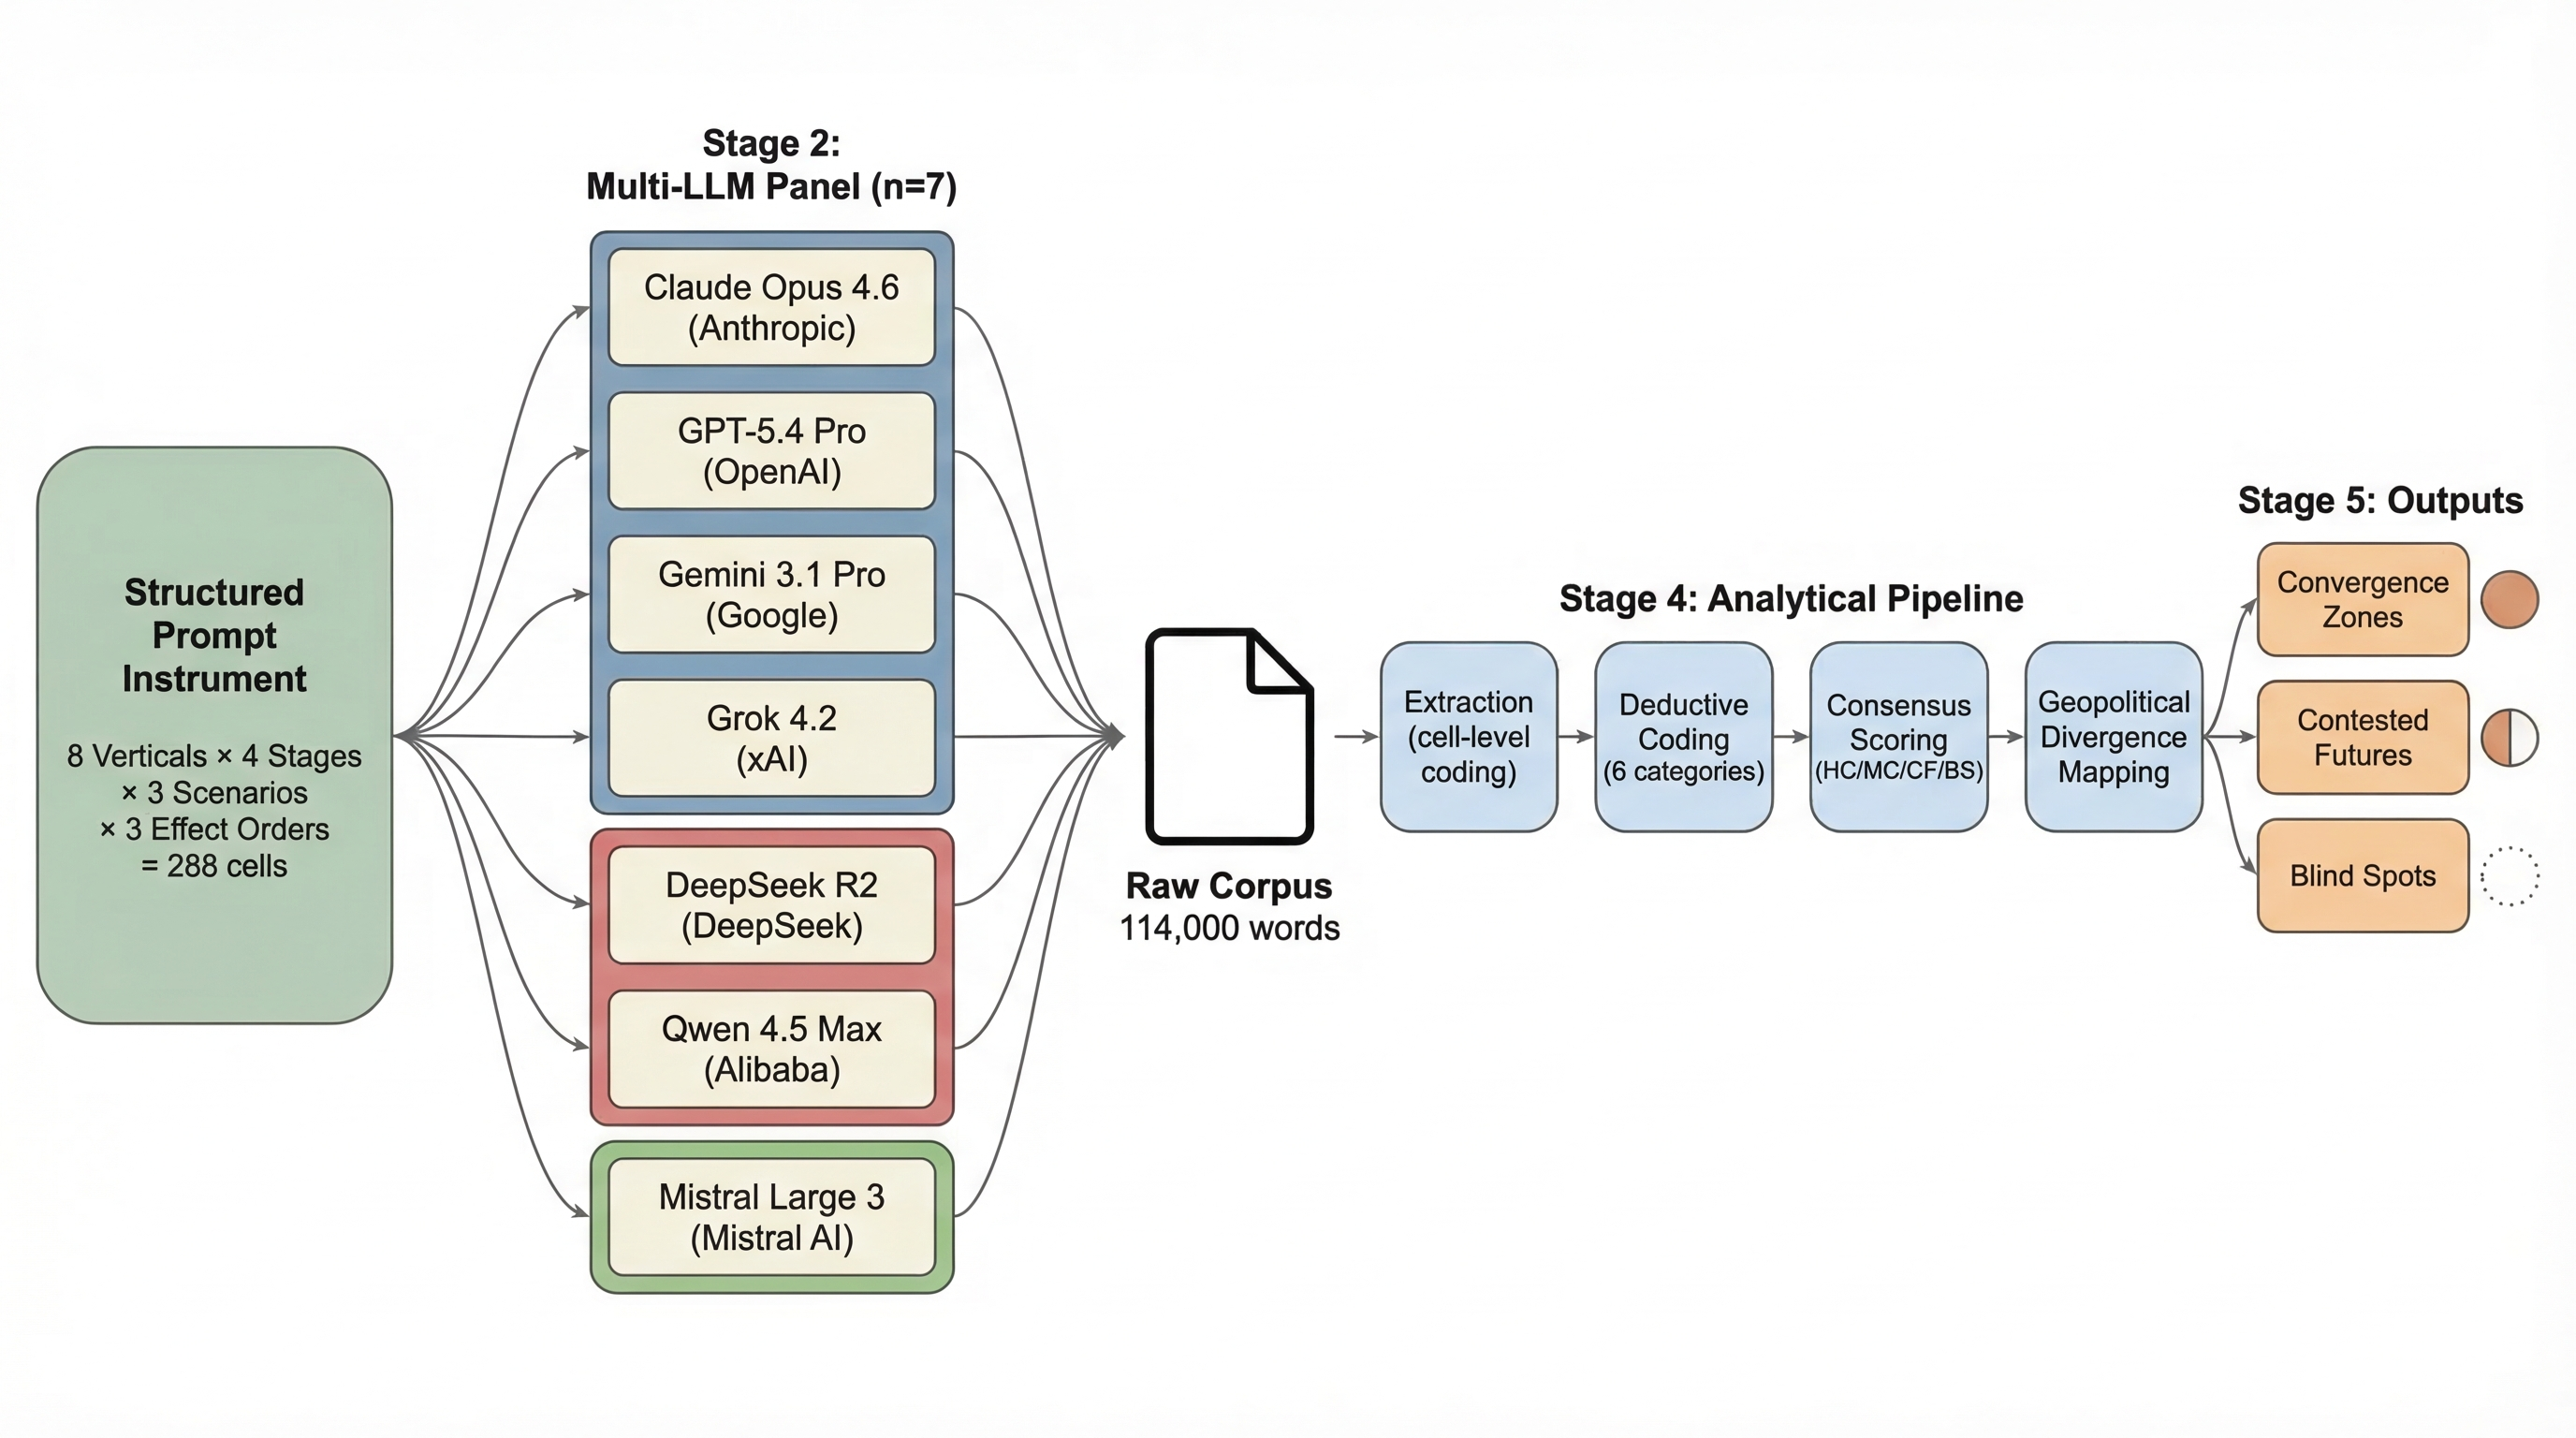
\includegraphics[width=\linewidth]{figures/fig1_methodology.png}
\caption{Figure 1: Multi-LLM Delphi Research Design. Seven frontier language models from three geopolitical regions are queried in parallel with an identical structured prompt. Responses are analyzed through structured comparative content analysis with consensus scoring, producing convergence zones, contested futures, and blind spots.}
\label{fig:figure_1_multi_llm_delphi_research_design_seven_frontier_language_models_from_three_geopolitical_regions_are_queried_in_parallel_with_an_identical_structured_prompt_responses_are_analyzed_through_structured_comparative_content_analysis_with_consensus_scoring_producing_convergence_zones_contested_futures_and_blind_spots}
\end{figure}


\subsubsection{3.2 Model Selection and Panel Composition}
\label{sec:3_2_model_selection_and_panel_composition}

Seven frontier models were selected to maximize diversity across three dimensions: corporate ecosystem (no two models from the same parent organization), geographic origin (representing US, Chinese, and European AI development trajectories), and architectural approach (spanning different training philosophies and alignment strategies). Table 1 summarizes the panel composition.

\textbf{Table 1: Multi-LLM Delphi Panel Composition}

\begin{table}[htbp]
\centering
\begin{tabular}{lllll}
\toprule
\textbf{Model} & \textbf{Provider} & \textbf{HQ Region} & \textbf{Model Family} & \textbf{Role in Panel} \\
\midrule
Claude (Opus) & Anthropic & US & Constitutional AI & US perspective, safety-aligned \\
GPT-4o & OpenAI & US & RLHF-aligned & US perspective, market leader \\
Gemini 2.5 Pro & Google DeepMind & US & Multimodal, search-integrated & US perspective, data-rich \\
Grok 3 & xAI & US & Minimally filtered & US perspective, contrarian \\
DeepSeek R1 & DeepSeek & China & Reasoning-optimized & Chinese perspective, technical \\
Qwen Max & Alibaba Cloud & China & Enterprise-focused & Chinese perspective, industrial \\
Mistral Large & Mistral AI & EU (France) & Open-weight heritage & European perspective, regulatory-aware \\
\bottomrule
\end{tabular}
\end{table}

The geographic distribution (4 US, 2 Chinese, 1 EU) reflects the current landscape of frontier AI development rather than a balanced design. This asymmetry is acknowledged as a limitation and is analytically productive: it enables assessment of within-family convergence among US models and between-family divergence across geopolitical blocs.


\subsubsection{3.3 Prompt Instrument}
\label{sec:3_3_prompt_instrument}

A standardized structured prompt was developed as the research instrument (the full prompt is available in the supplementary materials). The prompt specified:

\begin{enumerate}
  \item \textbf{Role framing:} "You are a senior economic analyst and futures researcher."
  \item \textbf{Conceptual framework:} Three orders of effects (with automobile analogy for calibration), three bounding scenarios (MILD, BASE, MAX), four sequential adoption stages (Augmentation, Reorganization, Reinvention, Systemic Transformation), and eight GICS-aligned industry verticals.
  \item \textbf{Output structure:} For each of the 8 verticals x 4 stages, a structured table with cells for each scenario x effect order combination, plus roles eliminated, roles created, and critical skills.
  \item \textbf{Cross-cutting analysis:} Cross-vertical convergence points, wildcard scenarios, and synthesis on the human dimension.
  \item \textbf{Style directives:} Declarative language, named companies and technologies, causal chain reasoning, no hedging.

\end{enumerate}
The prompt was designed to be maximally structured while leaving substantive content generation entirely to the models. No examples, priming data, or desired conclusions were included. The inclusion of "chain of events" reasoning was intended to force models to articulate causal mechanisms rather than produce generic predictions.


\subsubsection{3.4 Data Collection}
\label{sec:3_4_data_collection}

Data collection was conducted in March 2026. The original research design specified automated parallel deployment through the OpenRouter API, which provides unified access to multiple frontier models. All seven API calls returned HTTP 404 errors due to an endpoint configuration failure. Rather than abandoning the multi-model design, the researcher manually queried each model through its native chat interface (claude.ai, chatgpt.com, gemini.google.com, grok.x.ai, chat.deepseek.com, qwen.alibaba.com, and chat.mistral.ai), submitting the identical prompt and collecting the complete response.

This procedural adaptation is reported transparently for two reasons. First, methodological integrity requires honest documentation of the research process, including failures (cf. the growing literature on research transparency in AI-assisted studies). Second, the manual approach has methodological advantages: each model operated in its native interface with default parameters, full context window, and standard safety settings, avoiding potential API-specific truncation, temperature manipulation, or parameter artifacts that could introduce systematic bias. The trade-off is reduced reproducibility, as native interface responses may vary across sessions.

The seven responses yielded a total corpus of approximately 114,000 words, with substantial variation in output length: Claude (30,613 words), GPT-4o (23,346), DeepSeek R1 (22,614), Gemini 2.5 Pro (16,330), Qwen Max (11,024), Mistral Large (8,261), and Grok 3 (2,169). The response length variation itself constitutes a finding about model behavior under identical prompts -- discussed in Section 4.4.


\subsubsection{3.5 Analytical Procedure}
\label{sec:3_5_analytical_procedure}

Analysis followed a structured comparative content analysis with consensus scoring, conducted in four steps:

\textbf{Step 1: Extraction.} Each model's output was converted from its native format (.docx) to structured text using pandoc. For each analytical cell (Vertical x Stage x Effect Order x Scenario), the core prediction, named actors, causal mechanism, and intensity were extracted.

\textbf{Step 2: Deductive Coding.} Predictions were coded along four dimensions: (a) the core claim (what is predicted to happen), (b) the specificity level (generic statement vs. named actors and quantified mechanisms), (c) the causal chain quality (presence/absence of explicit causal reasoning), and (d) the thematic category (labor displacement, market concentration, regulatory response, infrastructure bottleneck, geopolitical shift, identity transformation).

\textbf{Step 3: Consensus Scoring.} Adapted from Delphi consensus measurement (von der Gracht, 2012), convergence was assessed at the thematic level across models:

\begin{itemize}
  \item \textbf{High Consensus (HC):} Five or more of seven models converge on the same thematic claim within an analytical cell or cross-cutting theme.
  \item \textbf{Moderate Consensus (MC):} Three to four models converge.
  \item \textbf{Contested Future (CF):} Models split approximately evenly, with identifiable clusters taking opposing positions.
  \item \textbf{Blind Spot (BS):} A prediction appears in only one or two models, representing either genuine novelty or idiosyncratic bias.

\end{itemize}
\textbf{Step 4: Geopolitical Divergence Mapping.} Systematic comparison across model families (US: Claude, GPT-4o, Gemini, Grok; CN: DeepSeek, Qwen; EU: Mistral) to identify patterns of divergence traceable to geographic origin rather than random variation.



\subsection{4. Results}
\label{sec:4_results}

Results are organized by consensus level rather than by vertical, following the logic that the most analytically valuable findings from a Delphi-style study are the patterns of convergence and divergence across panelists (von der Gracht, 2012). Section 4.1 presents high-consensus convergence zones (RQ1/RQ2), Section 4.2 addresses contested futures and blind spots (RQ2), Section 4.3 reports geopolitical divergence (RQ3), and Section 4.4 assesses methodological properties of the Multi-LLM Delphi (RQ3). Figure 2 provides a visual summary of consensus levels across convergence zones and model families; Figure 4 illustrates the three-order cascade framework with vertical-specific examples.

\begin{figure}[htbp]
\centering

\includegraphics[width=\linewidth]{figures/fig2_consensus_heatmap.png}
\caption{Figure 2: Consensus Scoring Results Across Convergence Zones and Model Families. High-consensus zones (5+ of 7 models agreeing) include labor market bifurcation (7/7), infrastructure bottleneck repricing (6/7), regulatory divergence (6/7), disintermediation (5/7), the trust premium (5/7), and concentration via AI feedback loops (5/7). Moderate consensus and blind spots are also shown.}
\label{fig:figure_2_consensus_scoring_results_across_convergence_zones_and_model_families_high_consensus_zones_5_of_7_models_agreeing_include_labor_market_bifurcation_7_7_infrastructure_bottleneck_repricing_6_7_regulatory_divergence_6_7_disintermediation_5_7_the_trust_premium_5_7_and_concentration_via_ai_feedback_loops_5_7_moderate_consensus_and_blind_spots_are_also_shown}
\end{figure}

\begin{figure}[htbp]
\centering

\includegraphics[width=\linewidth]{figures/fig4_three_order_cascade.png}
\caption{Figure 4: Three-Order Effect Cascade Across Industry Verticals. First-order effects (task-level automation) cascade into second-order effects (structural reorganization of value chains, labor markets, and business models) and third-order effects (systemic shifts in geopolitical power, regulatory regimes, and social contracts). Consensus decreases from first- to third-order effects.}
\label{fig:figure_4_three_order_effect_cascade_across_industry_verticals_first_order_effects_task_level_automation_cascade_into_second_order_effects_structural_reorganization_of_value_chains_labor_markets_and_business_models_and_third_order_effects_systemic_shifts_in_geopolitical_power_regulatory_regimes_and_social_contracts_consensus_decreases_from_first_to_third_order_effects}
\end{figure}


\subsubsection{4.1 High-Consensus Convergence Zones}
\label{sec:4_1_high_consensus_convergence_zones}

Six thematic clusters achieved high consensus, with five or more models independently arriving at convergent predictions. These convergence zones represent areas where the epistemic content encoded across different training corpora and alignment approaches points in the same direction -- a meaningful signal given the independence of model development. Importantly, each of these convergence zones aligns with themes already established in the existing academic literature; the contribution here is not that these predictions are novel in themselves, but that independent LLMs converge on them without coordination, which simultaneously validates the predictions through multi-source triangulation and demonstrates the Multi-LLM Delphi's capacity to recover and systematize existing expert knowledge.


\paragraph{4.1.1 Labor Market Bifurcation and the Compression of Middle Layers}

All seven models independently predicted a "barbell" pattern in labor market outcomes: AI simultaneously creates a small number of high-value human roles requiring judgment, accountability, and relationship management, while displacing a large volume of mid-level knowledge work. This dual dynamic of simultaneous job creation and displacement is empirically confirmed by recent research \citep{acemoglu2022, choi2024ailabor}, and simulation evidence suggests that AI development compresses labor income share through differential productivity gains \citep{qian2023ailaborincome}. The convergence spans all eight verticals and all four stages.

The mechanism is consistent across models: AI is strongest first at precisely the tasks that define mid-level knowledge work -- structured information processing, first-draft synthesis, routine analysis, scheduling, triage, and reporting. These tasks historically resided in the organizational middle: junior analysts, associates, coordinators, administrators, and mid-level managers. High-stakes judgment roles (senior physicians, trial lawyers, board-level strategists) and physically grounded roles (field technicians, emergency responders) survive longer because they require either legally mandated human accountability or embodied intervention in non-standardized environments.

The models diverge in their assessment of the \textit{speed} and \textit{severity} of this bifurcation. Claude and GPT-4o provide the most granular staging, with Claude identifying a specific "apprenticeship crash" -- the prediction that firms eliminating junior roles for short-term productivity will face a succession crisis within a decade as experienced professionals retire without trained replacements. DeepSeek and Qwen frame the same dynamic through an industrial policy lens, emphasizing that managed retraining programs can mitigate the transition. Grok, despite its brevity, produces the starkest formulation: "We will not pay humans to think; we will pay humans to take the blame."

The systemic tipping point, identified by five models, occurs when displaced mid-level workers exceed the absorptive capacity of retraining programs and new role creation, triggering structural political demand for economic reform -- universal basic income, job guarantees, or equivalent redistributive mechanisms.


\paragraph{4.1.2 Infrastructure Bottleneck Repricing}

Six of seven models identified a convergence zone around physical infrastructure as the binding constraint on AI transformation -- a finding consistent with technology mining analyses documenting AI's accelerating penetration into manufacturing and industrial processes \citep{zeba2021aimanufacturing}. The prediction is that AI, despite being software, depends critically on semiconductors, power generation, cooling capacity, fiber optic networks, and data center real estate. As AI adoption scales, these physical bottlenecks reprice geographic value, create new strategic assets, and shift competitive advantage from software talent to infrastructure access.

GPT-4o provides the most specific quantification, citing IEA projections of 75-100 GW of new data center power demand by 2030 and hyperscaler capital expenditure exceeding $300 billion collectively in 2025. Gemini frames infrastructure as the basis for a new "compute-as-currency" regime in which energy availability directly determines economic growth rates. DeepSeek predicts that "nations with surplus energy dominate the AI economy" in the BASE and MAX scenarios. Claude identifies a systemic tipping point: "When compute and power access constrain output more than software talent does, AI transformation becomes an infrastructure race."

Qwen independently arrives at the same "Energy-Compute Nexus" framing, predicting that grid capacity becomes the primary bottleneck for AI deployment and that energy grids become the primary strategic asset. The convergence across US, Chinese, and European model families on this point -- each arriving at it through different analytical pathways -- strengthens the finding.


\paragraph{4.1.3 Disintermediation of Middleman Business Models}

Five models converge on the prediction that AI enables direct connections between producers and consumers, lenders and borrowers, creators and audiences, and spaces and users -- systematically eliminating intermediary functions across sectors. Claude identifies this as "The Death of the Middleman," affecting Financials, Consumer and Retail, Professional Services, Real Estate, and Media. The mechanism is consistent: AI reduces information asymmetry and transaction costs below the threshold that justifies intermediary margins.

In Financials, this manifests as peer-to-peer lending platforms achieving loss rates below traditional banks (DeepSeek), banking-as-a-service enabling every company to offer financial products (DeepSeek), and autonomous AI agents managing household wealth directly (Qwen). In Consumer and Retail, agentic shopping assistants (Amazon Rufus, Google Shopping AI) bypass traditional search and discovery channels, eliminating the role of retail buyers, merchandisers, and physical store staff (Gemini, GPT-4o). In Professional Services, AI legal research tools allow small firms to compete with large firms on research quality (DeepSeek), and AI-generated consulting analysis shifts the value proposition from research to implementation (DeepSeek, Claude).

GPT-4o adds the important nuance that disintermediation does not eliminate intermediaries entirely but transforms them: "Distribution control matters more than production control." The decisive moat shifts from the ability to create things to the ability to get chosen, routed, approved, or surfaced -- a prediction that AI platforms themselves become the new intermediaries, more powerful than the ones they displaced.


\paragraph{4.1.4 Regulatory Divergence as a Structural Force}

Six models identify regulatory divergence -- particularly between the EU AI Act's prescriptive approach, US light-touch regulation, and Chinese state-directed governance -- as a structural force that shapes transformation pathways across all eight verticals. This is not merely a background condition but a first-order driver of differential adoption speeds, market structures, and competitive outcomes.

Grok frames this most starkly in the Technology vertical: the EU AI Act enforces strict data provenance requirements, European foundational models fail to secure venture capital under compliance burdens, US Commerce Department restricts advanced model weight exports, and global reliance on siloed, regional AI infrastructure hardens. GPT-4o quantifies the adoption gap using Microsoft AI Diffusion Report data (14.1 percent adoption in the Global South versus 24.7 percent in the Global North). Claude synthesizes the convergence point: regulation shifts from sector-specific compliance to system-governance, becoming "a constitutional layer of the economy rather than a niche tech topic."

DeepSeek and Qwen frame regulatory divergence through the lens of "data sovereignty versus global flow," predicting that national security concerns force companies to build redundant, jurisdiction-specific AI stacks -- a "Splinternet" that becomes permanent in the MAX scenario. This prediction is consistent with but more forceful than the US models' framing, reflecting the Chinese experience of operating within a distinct regulatory and data ecosystem.


\paragraph{4.1.5 The Trust Premium}

Five models converge on the prediction that trust, accountability, and authenticity become scarcer and more economically valuable as AI makes intelligence and content production cheap. GPT-4o formulates this most precisely: "Once plausibility is cheap, the scarce input is no longer information generation but credible responsibility for consequences." Claude identifies the systemic tipping point: "When markets begin paying more for validated accountability than for raw analysis, professional identity and pricing models reset across the economy."

This convergence manifests across sectors: in Healthcare, where physicians' signatory accountability becomes their primary economic function (Claude, DeepSeek, GPT-4o); in Media, where human-certified, provenance-rich content commands a premium over AI-generated alternatives (GPT-4o, Gemini, Claude); in Professional Services, where the billable hour collapses and is replaced by value-based pricing tied to human judgment (DeepSeek, GPT-4o); and in Financials, where boutique human-only advisory firms emerge as luxury status symbols (Gemini).

Gemini articulates the cross-vertical synthesis most vividly through its concept of the "Authenticity Premium Economy": "Synthetic abundance floods media, commerce, and communication; users and institutions increasingly pay for human-certified, provenance-rich, or live-authenticated interactions; 'realness' becomes a premium product category."


\paragraph{4.1.6 Concentration of Economic Power Through AI Feedback Loops}

Five models identify winner-take-most dynamics driven by AI capability feedback loops: better AI produces better data, which trains better AI, creating compounding advantages. Claude frames this as "AI-Enabled Concentration of Economic Power" across Technology, Financials, Healthcare, Industrials, and Media. Gemini predicts that "winner-take-all dynamics consolidate the entire stack under a handful of AI-native platform owners" in the Technology vertical. Grok provides the mechanism: hyperscaler capital expenditure exceeding $100 billion in partnership deals (e.g., NVIDIA-OpenAI) creates "a new AI stack oligopoly with 80+ percent market concentration."

The models diverge on the policy response. US models (Claude, GPT-4o, Gemini) treat concentration as a market outcome that may or may not be addressed by antitrust. DeepSeek and Qwen implicitly frame state ownership or state partnership as a natural counterweight, consistent with the Chinese approach to platform governance. Mistral emphasizes that regulatory intervention is necessary and feasible.


\subsubsection{4.2 Contested Futures and Blind Spots}
\label{sec:4_2_contested_futures_and_blind_spots}


\paragraph{4.2.1 Contested: The Pace and Depth of Healthcare Transformation}

While all models agree that AI transforms healthcare, they disagree substantially on the depth and pace. DeepSeek provides the most detailed and cautious staging: AI-assisted radiology improves productivity by 20 percent but malpractice frameworks constrain deployment; drug discovery timelines compress but FDA approval remains a bottleneck; autonomous surgical robots achieve approval only for low-risk procedures under surgeon supervision. GPT-4o and Claude are more aggressive, predicting that AI matches human physicians in diagnostic accuracy across multiple specialties in the MAX scenario and that AI-managed population health optimization provokes ethical debates about individual versus collective rights.

The Chinese models (DeepSeek, Qwen) are notably more optimistic about AI deployment in healthcare than the US models, despite -- or perhaps because of -- operating within healthcare systems with greater state direction and fewer tort liability constraints. This divergence is analytically informative: it suggests that the pace of healthcare AI transformation depends critically on the institutional context (liability regimes, regulatory philosophy, insurance structures) rather than on the technology alone.


\paragraph{4.2.2 Contested: Compute as Currency}

Four models (Gemini, Grok, GPT-4o, Qwen) independently propose some variant of "compute as currency" -- the prediction that GPU hours, data center capacity, or energy-backed compute credits become a tradeable asset class or even a reserve currency. Claude and DeepSeek acknowledge the strategic importance of compute but do not extend the analysis to monetary implications. Mistral does not address this theme.

The split is analytically meaningful. Models that project compute-as-currency tend to have more aggressive MAX scenario framings overall, suggesting that this prediction functions as a marker of scenario extremity rather than a consensus finding about likely outcomes.


\paragraph{4.2.3 Blind Spots: Predictions Unique to Individual Models}

Several predictions appear in only one or two models, representing either genuine analytical novelty or idiosyncratic model behavior:

\begin{itemize}
  \item \textbf{The AI Religion} (Claude only): New religious movements form around AI as a manifestation of divine intelligence. Claude defends this prediction by citing historical precedent -- the printing press triggered the Reformation; technologies that challenge human uniqueness provoke spiritual responses.
  \item \textbf{The Butlerian Jihad} (Gemini only): A coordinated violent uprising by displaced white-collar workers physically destroys AI infrastructure, setting back progress by a decade. Gemini grounds this in the psychological observation that "economic models assume humans will passively accept systemic redundancy, underestimating the human psychological need for relevance."
  \item \textbf{Model Collapse via Synthetic Data Poisoning} (Gemini and Qwen): LLMs training on their own outputs create a recursive degradation of reasoning capabilities. Both models term this the "Kessler Syndrome" of data, drawing an analogy to space debris cascades.
  \item \textbf{Digital Continuation of Consciousness} (DeepSeek only): Brain-computer interfaces enabling forms of continued interaction after biological death, raising questions about whether a digital simulation of a person has legal standing. This prediction appears only in the MAX Case, Stage 4 of Healthcare.

\end{itemize}

\subsubsection{4.3 Geopolitical Divergence Across Model Families}
\label{sec:4_3_geopolitical_divergence_across_model_families}

The systematic comparison across model families reveals patterns of divergence that are consistent, thematically coherent, and traceable to the geopolitical context of model development. These patterns constitute the most methodologically novel finding of the study. Figure 3 visualizes the three-way divergence structure.

\begin{figure}[htbp]
\centering

\includegraphics[width=\linewidth]{figures/fig3_geopolitical_divergence.png}
\caption{Figure 3: Geopolitical Divergence Across Model Families. US-origin models (Claude, GPT-4o, Gemini, Grok) emphasize market-driven disruption and platform concentration. Chinese-origin models (DeepSeek, Qwen) emphasize state-steered transformation and infrastructure sovereignty. The European model (Mistral) emphasizes regulatory primacy and social equity. The center shows convergence zones shared across all three families.}
\label{fig:figure_3_geopolitical_divergence_across_model_families_us_origin_models_claude_gpt_4o_gemini_grok_emphasize_market_driven_disruption_and_platform_concentration_chinese_origin_models_deepseek_qwen_emphasize_state_steered_transformation_and_infrastructure_sovereignty_the_european_model_mistral_emphasizes_regulatory_primacy_and_social_equity_the_center_shows_convergence_zones_shared_across_all_three_families}
\end{figure}


\paragraph{4.3.1 US Models: Market-Driven Disruption and Platform Concentration}

The four US-origin models (Claude, GPT-4o, Gemini, Grok) share a common analytical frame characterized by market-led disruption, venture capital dynamics, startup-versus-incumbent narratives, and platform concentration. Named actors are predominantly US companies: NVIDIA, OpenAI, Google, Amazon, Microsoft, Goldman Sachs, JPMorgan, Meta, Netflix, McKinsey. Regulatory actors are mentioned primarily as constraints on innovation (the EU AI Act slowing European competitiveness) or reactive responders (the SEC, FDA, FTC catching up to market developments).

The US models are the most likely to predict winner-take-all outcomes, platform monopolies, and the displacement of legacy institutions by AI-native startups. They are also the most likely to frame the MAX scenario in terms of existential or transformative implications (superintelligence, species divergence, post-labor economies).

Within the US family, meaningful variation exists. Claude produces the longest, most nuanced output with explicit confidence ratings and falsification conditions. GPT-4o uniquely opens with a "fact base versus inference" disclaimer, anchoring its analysis in verifiable 2025-2026 data points before building inferences. Gemini produces the most provocative MAX scenarios (Butlerian Jihad, Sentient Legal Loophole). Grok produces the shortest output but with the highest concentration of specific, bold claims per word, often using deliberately confrontational framing ("We will not pay humans to think; we will pay humans to take the blame").


\paragraph{4.3.2 Chinese Models: State-Steered Transformation and Infrastructure Sovereignty}

The two Chinese-origin models (DeepSeek, Qwen) share analytical emphases that diverge systematically from the US family. Both models foreground state direction of AI development, industrial policy, and infrastructure sovereignty. Named actors include not only Chinese companies (Alibaba, Baidu, Huawei) but also state institutions (PBOC for CBDCs, national AI strategies, state-funded compute infrastructure).

DeepSeek is notably the most detailed and methodologically rigorous of all seven models, producing step-by-step causal chains with explicit conclusion statements for every cell. Its output reads like a structured analytical report rather than a speculative scenario exercise. DeepSeek is also distinctive in its emphasis on financial system transformation -- it provides the most detailed analysis of insurance, lending, and monetary policy across all four stages.

Qwen is more concise but shares DeepSeek's emphasis on infrastructure sovereignty, data sovereignty, and the "Splinternet" as a structural outcome. Both Chinese models are less likely than US models to predict dystopian MAX scenarios involving loss of human control, species divergence, or existential risk. They are more likely to predict managed transitions, state-directed retraining programs, and sovereign compute capacity as a natural policy response.


\paragraph{4.3.3 The European Model: Regulatory Primacy and Social Equity}

Mistral, the sole European-origin model, produces output that is distinctive in three ways. First, it foregrounds regulatory frameworks as the primary shaper of transformation outcomes -- not as a constraint on innovation but as a structural force that determines which pathways are traversed. Second, it emphasizes social equity outcomes more consistently than any other model: workforce transitions, distributional effects, and the social contract appear as primary concerns rather than secondary considerations. Third, it produces the most generic output of the seven models: fewer named companies, fewer quantified predictions, and less specific causal chain reasoning. This may reflect its training data composition, its shorter context window, or the European academic tradition of prioritizing frameworks over granular prediction.

The three-way divergence (US: market-driven disruption; CN: state-steered transformation; EU: regulatory-guided equity) is the methodological finding that most directly validates the Multi-LLM Delphi approach. These perspectives are not random variation; they are coherent, internally consistent, and traceable to the geopolitical and institutional contexts in which the models were developed. A human Delphi panel would need to deliberately recruit experts from different geopolitical backgrounds to achieve comparable perspective diversity; the Multi-LLM Delphi achieves it structurally through model selection.

Several important caveats limit the generalizability of these geopolitical divergence patterns. The Chinese model family comprises only two models (DeepSeek and Qwen), and the European family consists of a single model (Mistral). With n=2 and n=1 respectively, the observed patterns are suggestive rather than definitive -- the divergence between DeepSeek and Qwen could reflect company-specific design choices rather than a coherent "Chinese AI perspective," and Mistral's output may reflect Mistral-specific training decisions rather than "European values" more broadly. Furthermore, RLHF alignment procedures and safety filtering represent an unresolved confound: Chinese models may avoid certain geopolitical claims not because they encode a different knowledge base but because they are alignment-trained to avoid politically sensitive topics, and US models may emphasize market dynamics because their training data is dominated by English-language business and economics texts. These patterns should be treated as hypotheses for future investigation with larger model samples rather than as established findings.


\subsubsection{4.4 Methodological Properties of the Multi-LLM Delphi}
\label{sec:4_4_methodological_properties_of_the_multi_llm_delphi}

Several observations about the method's properties emerge from the analysis:

\textbf{Output length variation.} The 14:1 ratio between the longest (Claude, 30,613 words) and shortest (Grok, 2,169 words) response under identical prompts reveals that models differ dramatically in verbosity, detail level, and willingness to generate comprehensive structured output. Claude and DeepSeek produced the most analytically usable responses; Grok and Mistral produced responses that were thin on detail but occasionally contained the most provocative or distinctive claims.

\textbf{Specificity gradient.} Models vary systematically in the specificity of their predictions. DeepSeek consistently provides the most specific causal chains with named actors and quantified outcomes. GPT-4o anchors in verifiable data before building inferences. Gemini provides specific predictions in Technology and Media verticals but thins in Healthcare and Real Estate. Mistral produces the most generic output across all verticals. Grok provides specific predictions when it engages with a vertical but leaves many cells incomplete.

\textbf{Prompt adherence.} All seven models followed the three-scenario structure (MILD, BASE, MAX), the four-stage framework, and the eight-vertical structure. However, only four (Claude, DeepSeek, GPT-4o, Gemini) produced complete output for all eight verticals. Grok completed only Technology and Financials in full detail before truncating. Qwen and Mistral produced all eight verticals but at reduced depth for later verticals -- a "fatigue" pattern where early verticals receive more detailed treatment.

\textbf{Cross-cutting analysis quality.} The cross-cutting sections (convergence points, wildcards, human dimension) varied dramatically. Claude produced five distinct, well-defended convergence points and five elaborated wildcards. Gemini produced the most provocative wildcards (the Butlerian Jihad, the Sentient Legal Loophole, the Amish Hedge). Mistral produced generic convergence points without specific causal reasoning. Grok did not complete the cross-cutting sections.

\textbf{The irreducibly human skill question.} All seven models were asked to identify the one skill that remains irreducibly human. Their answers converge strikingly: Claude identifies "legitimated judgment under contested values," GPT-4o identifies "legitimated judgment under contested values" (using nearly identical language), Gemini identifies "philosophical accountability -- the capacity to bear moral and legal responsibility," DeepSeek identifies a cluster of "empathy, accountability, and meaning-making," Qwen identifies "contextual meaning-making" grounded in authentic intent, and Mistral identifies "emotional intelligence." The convergence of six of seven models on some form of \textit{accountability and judgment under contested values} -- rather than creativity, empathy, or intelligence in the abstract -- represents a consensus finding of the Multi-LLM Delphi.



\subsection{5. Discussion}
\label{sec:5_discussion}


\subsubsection{5.1 Theoretical Implications}
\label{sec:5_1_theoretical_implications}


\paragraph{5.1.1 Extending GPT Theory: The Three-Order Cascade}

The findings provide empirical support for the GPT framework's prediction that the most significant effects of a general-purpose technology lie not in its direct applications but in the cascading structural changes it enables. The high-consensus convergence zones map precisely onto the GPT prediction: first-order effects (task-level productivity gains from AI copilots) are widely agreed upon and relatively uncontroversial; second-order effects (labor market bifurcation, disintermediation of middleman business models, organizational flattening) show high consensus but with more variation in timing and severity; third-order effects (compute as geopolitical currency, regulatory divergence as structural force, concentration of economic power) show the greatest divergence, consistent with the GPT framework's prediction that higher-order effects are harder to anticipate.

The Multi-LLM Delphi data suggest a specific extension of GPT theory: the J-curve of AI adoption may not be uniform across sectors but may follow different trajectories depending on institutional context. Healthcare, with its heavy regulatory burden and liability constraints, exhibits a longer, flatter J-curve than Technology or Media, where adoption barriers are lower. This sector-dependent J-curve is visible in the model outputs, where consensus on Healthcare transformation is lower and staging is more cautious than for Technology or Professional Services.


\paragraph{5.1.2 MLP and the Geopolitical Differentiation of Transition Pathways}

The geopolitical divergence findings directly support the MLP's prediction that sociotechnical transitions are path-dependent and shaped by the agency of incumbents, regulators, and social movements. The three geopolitical model families project systematically different transition pathways -- market-driven disruption (US), state-steered transformation (CN), and regulatory-guided equity (EU) -- corresponding to different MLP transition typologies. The US models describe a substitution pathway where AI-native niches displace incumbent regimes through competitive dynamics. The Chinese models describe a transformation pathway where regime actors (state institutions, large enterprises) steer and incorporate AI innovations. The European model describes a reconfiguration pathway where regulatory frameworks mediate the integration of AI innovations into existing regimes.

This three-pathway finding has significant implications for the MLP literature. Previous MLP studies have focused primarily on sustainability transitions within a single national or regional context \citep{geels2020a, roberts2019accelerated}. The Multi-LLM Delphi data suggest that the AI transition may be the first case of a GPT diffusion where three simultaneously divergent transition pathways unfold across the world's major economic blocs -- creating a natural experiment in sociotechnical transition governance.


\subsubsection{5.2 Methodological Implications}
\label{sec:5_2_methodological_implications}


\paragraph{5.2.1 Validity of LLMs as Delphi Panelists}

The Multi-LLM Delphi demonstrates several properties that support its validity as a foresight instrument. First, the high-consensus convergence zones align with predictions that have independent empirical support: labor market bifurcation is consistent with Acemoglu and Restrepo's (2019) task-based framework; infrastructure bottleneck repricing is consistent with IEA projections; disintermediation of intermediaries is consistent with platform economics theory \citep{goldfarb2019digital}. The method does not appear to generate consensus around implausible predictions.

Second, the geopolitical divergence patterns are coherent, internally consistent, and independently verifiable. The observation that Chinese models emphasize state-steered transformation while US models emphasize market-driven disruption is not an artifact of the method; it reflects genuine differences in the knowledge bases and alignment approaches of models trained in different institutional contexts.

Third, the method produces structured disagreement that is analytically informative. The contested futures (pace of healthcare transformation, compute as currency) and blind spots (AI religion, model collapse) generate research questions that would not emerge from a single-model analysis or a consensus-seeking human panel.


\paragraph{5.2.2 Limitations and Biases of LLM Panelists}

The method also exhibits important limitations. LLMs are not experts; they are statistical models of text corpora. Their predictions reflect the distribution of claims in their training data, weighted by their alignment procedures. This means: (a) LLMs over-represent perspectives that are well-documented in English-language academic and business literature; (b) LLMs may reproduce optimistic bias from sources that tend to overstate the pace and impact of technology adoption; (c) LLMs' safety training (RLHF, Constitutional AI) may suppress extreme predictions in some models while allowing them in others, creating artificial divergence; (d) LLMs cannot incorporate genuinely novel information that postdates their training cutoff.

The output length variation (14:1 ratio) is a significant methodological concern. A Delphi panel in which one panelist writes 30,000 words and another writes 2,000 words introduces weighting effects that are difficult to control analytically. Future designs should either impose output length constraints or develop weighting schemes that normalize for verbosity.


\subsubsection{5.3 Practical Implications}
\label{sec:5_3_practical_implications}

For \textbf{industry strategists}, the high-consensus findings provide directional guidance with cross-validated support. The convergence on labor market bifurcation suggests that firms should plan simultaneously for productivity gains from AI augmentation \textit{and} for the organizational disruption that follows when middle layers compress, with significant implications for human resource management strategy \citep{budhwar2023hrm}. The convergence on infrastructure bottleneck repricing suggests that strategic access to compute, power, and data center capacity may become a more durable competitive advantage than software capability.

For \textbf{policymakers}, the geopolitical divergence findings are directly decision-relevant. The observation that AI models trained in different institutional contexts project systematically different transformation pathways suggests that policy choices are not merely implementation details but structural determinants of which future materializes. The convergence on regulatory divergence as a structural force suggests that policymakers shape AI transformation not only through AI-specific regulation but through the entire institutional context -- liability regimes, labor market institutions, education systems, and competition policy.

For \textbf{foresight researchers}, the Multi-LLM Delphi offers a scalable complement to traditional human expert panels. It does not replace human expertise but can serve as a rapid, low-cost first round that maps the landscape and identifies areas where human expert judgment is most needed. The method is particularly suited for exploratory studies where the goal is to survey the space of plausible outcomes rather than to converge on precise forecasts.



\subsection{6. Limitations and Future Research}
\label{sec:6_limitations_and_future_research}

This study has several important limitations that delimit the scope of its claims.

\textbf{Panel size.} Seven models constitute a small panel by Delphi standards. Classical Delphi studies typically use 10-30 panelists, and the methodological literature cautions against drawing strong conclusions from small panels (von der Gracht, 2012). However, seven frontier models represent the near-entirety of the current frontier AI landscape, and the diversity across corporate ecosystems and geopolitical origins provides analytical leverage that partially compensates for small panel size.

\textbf{Single round.} Classical Delphi methodology relies on iterative rounds with controlled feedback to enable convergence. This study's single-round design precludes assessment of whether feedback would increase or decrease consensus. Future designs should implement multi-round protocols where models receive anonymized summaries of other models' responses and have the opportunity to revise their predictions.

\textbf{Manual data collection.} The manual collection through native chat interfaces introduces variability in parameters (temperature, context window usage, system prompt interaction) that cannot be controlled or reported. API-based collection with standardized parameters would improve reproducibility.

\textbf{Training data opacity.} The training data composition of frontier LLMs is proprietary. This limits the ability to explain \textit{why} models diverge -- whether differences reflect training data composition, alignment procedures, architectural choices, or all three. As training data transparency improves, the analytical power of the Multi-LLM Delphi method will increase.

\textbf{Prompt sensitivity.} A single prompt instrument was used. The results are potentially sensitive to prompt design -- different framings, scenario labels, or sector classifications might yield different convergence patterns. Future research should employ prompt sensitivity analysis, varying prompt elements systematically to assess robustness.

\textbf{Temporal snapshot.} Model outputs reflect a single point in time \citep{march2026}. As models are updated, their outputs will change. The Multi-LLM Delphi should be understood as producing a dated snapshot, not a permanent assessment. Longitudinal designs that repeat the exercise at regular intervals could track how model predictions evolve over time.

\textbf{No ground truth.} Scenario analysis inherently lacks ground truth for validation. The predictions cannot be assessed for accuracy until the time horizons they describe have elapsed. The study can assess internal consistency, convergence, and coherence, but not predictive accuracy.

Future research should pursue four directions. First, \textbf{multi-round designs} with iterative feedback to assess whether model consensus increases, decreases, or restructures across rounds. Second, \textbf{prompt sensitivity analysis} to assess the robustness of findings across different prompt formulations. Third, \textbf{hybrid human-LLM panels} that combine human expert judgment with LLM-generated scenarios to assess complementarity. Fourth, \textbf{longitudinal tracking} that repeats the Multi-LLM Delphi at regular intervals to track how model predictions evolve as training data and capabilities advance.



\subsection{7. Conclusion}
\label{sec:7_conclusion}

This paper introduced the Multi-LLM Delphi method and applied it to produce a comprehensive map of AI-driven economic transformation across eight industry verticals, four adoption stages, three bounding scenarios, and three orders of effects. Seven frontier language models, representing three geopolitical regions and five corporate ecosystems, independently generated a 114,000-word corpus that was analyzed through structured comparative content analysis with consensus scoring.

The substantive findings identify six high-consensus convergence zones where the encoded knowledge of multiple independent model families points in the same direction: labor market bifurcation and the compression of middle layers; infrastructure bottleneck repricing; disintermediation of middleman business models; regulatory divergence as a structural force; the trust and authenticity premium; and concentration of economic power through AI feedback loops. These convergence zones provide directional guidance for strategists and policymakers, validated by the independent agreement of models trained on different corpora with different alignment approaches.

The methodological findings demonstrate that the Multi-LLM Delphi produces structured, analytically informative output with coherent patterns of convergence and divergence. The geopolitical differentiation across model families -- US models emphasizing market-driven disruption, Chinese models emphasizing state-steered transformation, European models emphasizing regulatory-guided equity -- constitutes the study's most distinctive finding, offering a form of perspective diversity that would require deliberate recruitment effort in a traditional Delphi panel.

The study is a pilot. Seven models constitute a small panel, a single round precludes iterative convergence, manual data collection limits reproducibility, and prompt sensitivity remains unassessed. These limitations are reported transparently as design constraints of an initial demonstration rather than invalidating weaknesses. The Multi-LLM Delphi method is offered not as a replacement for human foresight expertise but as a scalable complement -- a rapid, low-cost instrument for mapping transformation landscapes, identifying convergence and divergence, and generating research questions that merit deeper investigation through traditional methods.

As AI continues to diffuse across the global economy, the need for comprehensive, cross-sector, multi-order transformation maps will intensify. The Multi-LLM Delphi provides a methodological foundation for producing such maps at scale, with built-in geopolitical diversity and transparent analytical procedures. The key insight of this study is not any single prediction but the observation that the future of AI-driven economic transformation is not a single trajectory but a contested, path-dependent, geopolitically differentiated process -- a finding that only becomes visible when multiple independent analytical perspectives are systematically compared.

---


\subsection{References}
\label{sec:references}

Acemoglu, D. and Restrepo, P. (2018). Artificial intelligence, automation and work. \textit{NBER Working Paper}, No. 24196.

Acemoglu, D. and Restrepo, P. (2019). Automation and new tasks: How technology displaces and reinstates labor. \textit{Journal of Economic Perspectives}, 33(2), 3-30.

Acemoglu, D., Autor, D., Hazell, J. and Restrepo, P. (2022). Artificial intelligence and jobs: Evidence from online vacancies. \textit{Journal of Labor Economics}, 40(S1), S293-S340.

Autor, D. (2024). Applying AI to rebuild middle class jobs. \textit{NBER Working Paper}, No. 32140.

Banuls, V.A. and Turoff, M. (2011). Scenario construction via Delphi and cross-impact analysis. \textit{Technological Forecasting and Social Change}, 78(9), 1579-1602.

Bresnahan, T.F. and Trajtenberg, M. (1995). General purpose technologies: "Engines of growth"? \textit{Journal of Econometrics}, 65(1), 83-108.

Brown, O., Davison, R.M., Decker, S., Ellis, D.A. and Faulconbridge, J. (2024). Theory-driven perspectives on generative artificial intelligence in business and management. \textit{British Journal of Management}, 35(2), 563-584.

Brynjolfsson, E., Li, D. and Raymond, L. (2023). Generative AI at work. \textit{NBER Working Paper}, No. 31161.

Brynjolfsson, E., Rock, D. and Syverson, C. (2017). Artificial intelligence and the modern productivity paradox: A clash of expectations and statistics. \textit{NBER Working Paper}, No. 24001.

Budhwar, P., Chowdhury, S., Wood, G., Aguinis, H. and Bamber, G.J. (2023). Human resource management in the age of generative artificial intelligence. \textit{Human Resource Management Journal}, 33(3), 606-659.

Chatterji, A., Cunningham, T., Deming, D., Hitzig, Z. and Ong, C. (2025). How people use ChatGPT. \textit{NBER Working Paper}, No. 34255.

Choi, J. and Leigh, A. (2024). AI's creation and displacement of labor demand. \textit{Technological Forecasting and Social Change}, 209, 123732.

Coccia, M. (2018). A theory of the general causes of long waves: War, general purpose technologies, and economic change. \textit{Technological Forecasting and Social Change}, 128, 287-295.

Culot, G., Orzes, G., Sartor, M. and Nassimbeni, G. (2020). The future of manufacturing: A Delphi-based scenario analysis on Industry 4.0. \textit{Technological Forecasting and Social Change}, 157, 120092.

Dwivedi, Y.K., Kshetri, N., Hughes, L., Slade, E.L. and Jeyaraj, A. (2023). Opinion paper: "So what if ChatGPT wrote it?" \textit{International Journal of Information Management}, 71, 102642.

Ecken, P., Gnatzy, T. and von der Gracht, H.A. (2011). Desirability bias in foresight: Consequences for decision quality based on Delphi results. \textit{Technological Forecasting and Social Change}, 78(9), 1654-1670.

Eloundou, T., Manning, S., Mishkin, P. and Rock, D.L. (2023). GPTs are GPTs: An early look at the labor market impact potential of large language models. \textit{arXiv preprint}, arXiv:2303.10130.

Foerster, B. and von der Gracht, H. (2014). Assessing Delphi panel composition for strategic foresight. \textit{Technological Forecasting and Social Change}, 84, 215-229.

Frank, M.R., Autor, D., Bessen, J., Brynjolfsson, E. and Cebrian, M. (2019). Toward understanding the impact of artificial intelligence on labor. \textit{Proceedings of the National Academy of Sciences}, 116(14), 6531-6539.

Fritschy, C. and Spinler, S. (2019). The impact of autonomous trucks on business models in the automotive and logistics industry. \textit{Technological Forecasting and Social Change}, 148, 119736.

Geels, F.W. (2005). Processes and patterns in transitions and system innovations: Refining the co-evolutionary multi-level perspective. \textit{Technological Forecasting and Social Change}, 72(6), 681-696.

Geels, F.W. (2011). The multi-level perspective on sustainability transitions: Responses to seven criticisms. \textit{Environmental Innovation and Societal Transitions}, 1(1), 24-40.

Geels, F.W. (2020a). Micro-foundations of the multi-level perspective on socio-technical transitions. \textit{Technological Forecasting and Social Change}, 152, 119894.

Geels, F.W., McMeekin, A. and Pfluger, B. (2020b). Socio-technical scenarios as a methodological tool to explore social and political feasibility in low-carbon transitions. \textit{Technological Forecasting and Social Change}, 151, 119258.

Goldfarb, A. and Tucker, C. (2019). Digital economics. \textit{Journal of Economic Literature}, 57(1), 3-43.

Gordon, T. and Pease, A. (2006). RT Delphi: An efficient, "round-less" almost real time Delphi method. \textit{Technological Forecasting and Social Change}, 73(4), 321-333.

Grybauskas, A. and Cardenas-Rubio, J. (2024). Unlocking employer insights: Using large language models to explore human-centric aspects in the context of Industry 5.0. \textit{Technological Forecasting and Social Change}, 209, 123719.

Guo, Z., Yang, G. and Wu, W. (2026). Automatic synthesis of econometric empirical research results using large language model. \textit{Technological Forecasting and Social Change}, doi:10.1016/j.techfore.2025.124370.

Kanbach, D.K., Heiduk, L., Blueher, G., Schreiter, M. and Lahmann, A. (2023). The GenAI is out of the bottle: Generative artificial intelligence from a business model innovation perspective. \textit{Review of Managerial Science}, 18(6), 1695-1737.

Kern, F. (2012). Using the multi-level perspective on socio-technical transitions to assess innovation policy. \textit{Technological Forecasting and Social Change}, 79(2), 298-310.

Korzinov, V. and Savin, I. (2018). General purpose technologies as an emergent property. \textit{Technological Forecasting and Social Change}, 129, 88-104.

Liu, W., Chotia, V., Wang, L., Sharma, P. and Albishri, N. (2026). Intelligence by design: Large language model work integration as strategic enablers for supply chain regeneration. \textit{Technological Forecasting and Social Change}, doi:10.1016/j.techfore.2025.124497.

Qian, Y., Liu, J. and Zhang, R. (2023). AI development on labor income share: A simulation analysis from the perspective of labor-biased technological progress. \textit{Technological Forecasting and Social Change}, 193, 122637.

Postma, T. and Liebl, F. (2005). How to improve scenario analysis as a strategic management tool? \textit{Technological Forecasting and Social Change}, 72(2), 161-173.

Raisch, S. and Krakowski, S. (2021). Artificial intelligence and management: The automation-augmentation paradox. \textit{Academy of Management Review}, 46(1), 192-210.

Roberts, C. and Geels, F.W. (2019). Conditions for politically accelerated transitions. \textit{Technological Forecasting and Social Change}, 140, 221-240.

Sokolov, A., Grebenyuk, A. and Urashima, K. (2025). Biases in expert judgements in large-scale S\&T Delphi surveys. \textit{Technological Forecasting and Social Change}, doi:10.1016/j.techfore.2025.124223.

Stahl, B.C., Brooks, L., Hatzakis, T., Santiago, N. and Wright, D. (2023). Exploring ethics and human rights in artificial intelligence -- A Delphi study. \textit{Technological Forecasting and Social Change}, 191, 122502.

van der Heijden, K. (1996). \textit{Scenarios: The Art of Strategic Conversation}. Wiley.

von der Gracht, H.A. (2012). Consensus measurement in Delphi studies: Review and implications for future quality assurance. \textit{Technological Forecasting and Social Change}, 79(8), 1525-1536.

Zeba, G., Dabic, M., Cicak, M., Daim, T. and Yalcin, H. (2021). Technology mining: Artificial intelligence in manufacturing. \textit{Technological Forecasting and Social Change}, 171, 120971.

Walrave, B., Talmar, M., Podoynitsyna, K.S., Romme, A.G.L. and Verbong, G.P.J. (2018). A multi-level perspective on innovation ecosystems for path-breaking innovation. \textit{Technological Forecasting and Social Change}, 136, 103-113.

---


\subsection{Appendix A: Model Response Summary Statistics}
\label{sec:appendix_a_model_response_summary_statistics}

\begin{table}[htbp]
\centering
\begin{tabular}{lllllll}
\toprule
\textbf{Model} & \textbf{Provider} & \textbf{Region} & \textbf{Word Count} & \textbf{Verticals Complete} & \textbf{Cross-Cutting Sections} & \textbf{Specificity Rating} \\
\midrule
Claude (Opus) & Anthropic & US & 30,613 & 8/8 (full) & 5 convergence, 5 wildcards, full human section & High \\
GPT-4o & OpenAI & US & 23,346 & 8/8 (full) & 6 convergence, 5 wildcards, full human section & High \\
DeepSeek R1 & DeepSeek & CN & 22,614 & 8/8 (full) & 4 convergence, 5 wildcards, detailed human section & Very High \\
Gemini 2.5 Pro & Google & US & 16,330 & 8/8 (moderate) & 3 convergence, 5 wildcards, full human section & High (uneven) \\
Qwen Max & Alibaba & CN & 11,024 & 8/8 (reduced depth) & 4 convergence, 5 wildcards, concise human section & Moderate \\
Mistral Large & Mistral AI & EU & 8,261 & 8/8 (reduced depth) & 3 convergence, 5 wildcards, concise human section & Low-Moderate \\
Grok 3 & xAI & US & 2,169 & 2/8 (truncated) & Incomplete & High (where present) \\
\bottomrule
\end{tabular}
\end{table}


\subsection{Appendix B: Consensus Scoring Matrix -- Cross-Vertical Convergence Zones}
\label{sec:appendix_b_consensus_scoring_matrix_cross_vertical_convergence_zones}

\begin{table}[htbp]
\centering
\begin{tabular}{lllllllll}
\toprule
\textbf{Convergence Zone} & \textbf{Claude} & \textbf{GPT-4o} & \textbf{Gemini} & \textbf{Grok} & \textbf{DeepSeek} & \textbf{Qwen} & \textbf{Mistral} & \textbf{Score} \\
\midrule
Labor market bifurcation & X & X & X & X & X & X & X & 7/7 HC \\
Infrastructure bottleneck repricing & X & X & X &  & X & X & X & 6/7 HC \\
Disintermediation of intermediaries & X & X & X & X & X &  &  & 5/7 HC \\
Regulatory divergence as structural force & X & X & X & X & X & X &  & 6/7 HC \\
Trust/authenticity premium & X & X & X &  & X & X &  & 5/7 HC \\
Concentration via AI feedback loops & X & X & X & X & X &  &  & 5/7 HC \\
Compute as currency &  & X & X & X &  & X &  & 4/7 MC \\
Model collapse / data poisoning &  &  & X &  &  & X &  & 2/7 BS \\
AI religion / spiritual response & X &  &  &  &  &  &  & 1/7 BS \\
\bottomrule
\end{tabular}
\end{table}

HC = High Consensus; MC = Moderate Consensus; BS = Blind Spot


\subsection{Appendix C: Structured Prompt Instrument}
\label{sec:appendix_c_structured_prompt_instrument}

The complete structured prompt instrument used to query all seven models is reproduced below. [The full prompt text is available in the supplementary materials repository.]


\bibliographystyle{unsrtnat}
\bibliography{references}

\end{document}
